\subsection*{Financial models of communication\label{sec:financial-models-of-communication}}

This section analyzes communication from a financial perspective, focusing on two observations:
being late to a meeting is theft, 
and poorly written email and email to the wrong people has financial cost.
The point of raising these is to enable comparison with other investments the organization makes. Creating a cost model can help determine how much effort into improving what might otherwise seem like cultural issues.

\subsubsection*{Meeting time compared to theft}
% https://graphthinking.blogspot.com/2021/02/organizations-value-things-more-than.html

In large organizations there can be significant bureaucracy associated with even small purchases. A multi-step review process may be incurred for a \$200 acquisition. (Typically the cost of the review process in terms of person-hours spent isn't part of the calculus.)

Another measurement of value is that if an employee were to steal even \$200 worth of materials, the organization would likely punish that employee.

In the book High Output Management~\cite{1995_Grove}, Grove points out that those metrics apply to tangible goods, but not to people's time. Consider a meeting of 10 people and each person's cost is \$200 per hour. 
\marginpar{$>>$ Math}
A wasted meeting is not unusual and would not incur bureaucratic review processes. The cost to the organization is fiscally the same -- \$2000. Similarly, consider an employee who is late and causes a loss of productivity. Merely depriving the organization of \$200 worth of time is not punished in the same way theft is.

In practice, organizations default to meetings (even recurring meetings) rather than not meet. And being late (by a few minutes) to a meeting is commonly accepted. 
We can debate the differences between theft of materials and theft of time. The financial argument is the two are indistinguishable. 


\subsubsection*{Email is not free}

Bureaucracy as distributed knowledge and distributed decision-making requires communication. Because synchronous communication like phone calls, video calls, and in-person meetings is challenging to coordinate, written communication is widely used for asynchronous collaboration. Whether that written content is emails or text-based chat, writing is expensive.

The cost of email includes
\begin{itemize}
    \item Time spent writing (authorship).
    \item Time spent reading (readership).
    \item Infrastructure maintenance.
\end{itemize}

Those three factors can be quantified as variables. 
\marginpar{$>>$ Math}
\begin{multline}
\text{Cost per email} = 
(\text{hourly rate of writer})*(\text{time spent writing}) +\\
(\text{hourly rate of reader})*(\text{time spent reading})*(\text{number of readers})+\\
\frac{\text{annual salary of maintainer}}{\text{number of emails per year}} + \frac{\text{email server cost}}{\text{number of emails per year}}
\end{multline}
Plugging in some numbers, suppose an author charging \$50 per hour spends 5 minutes writing an email to 4 people. Each of those four people also charges \$50 per hour and spends 2 minutes on reading. 
\begin{equation}
50*(5/60) + 50*(2/60)*4 + \frac{100000}{1000000} + \frac{10000}{1000000} = \$10.84
\label{eq:four_readers}
\end{equation}
The cost to the organization is \$11 for one email! The breakdown of the three variables is shown in Figure~\ref{fig:my_label}. You've probably sent and received more than one email in your professional career as a bureaucrat. 


If the cost of one email doesn't lead you to be careful with communication, consider the cost to the organization of communication. If email consumes 2 hours a day per person (reading and writing), and if staffing is 50\% of the organization's budget, then 
    % (2/8)*0.5
12.5\% of the organization's budget is spent on email. The same math for applies to meetings, so with 2 hours of meeting and 2 hours of email that's 25\% of the organization's budget on coordination.

\begin{figure}
    \centering
    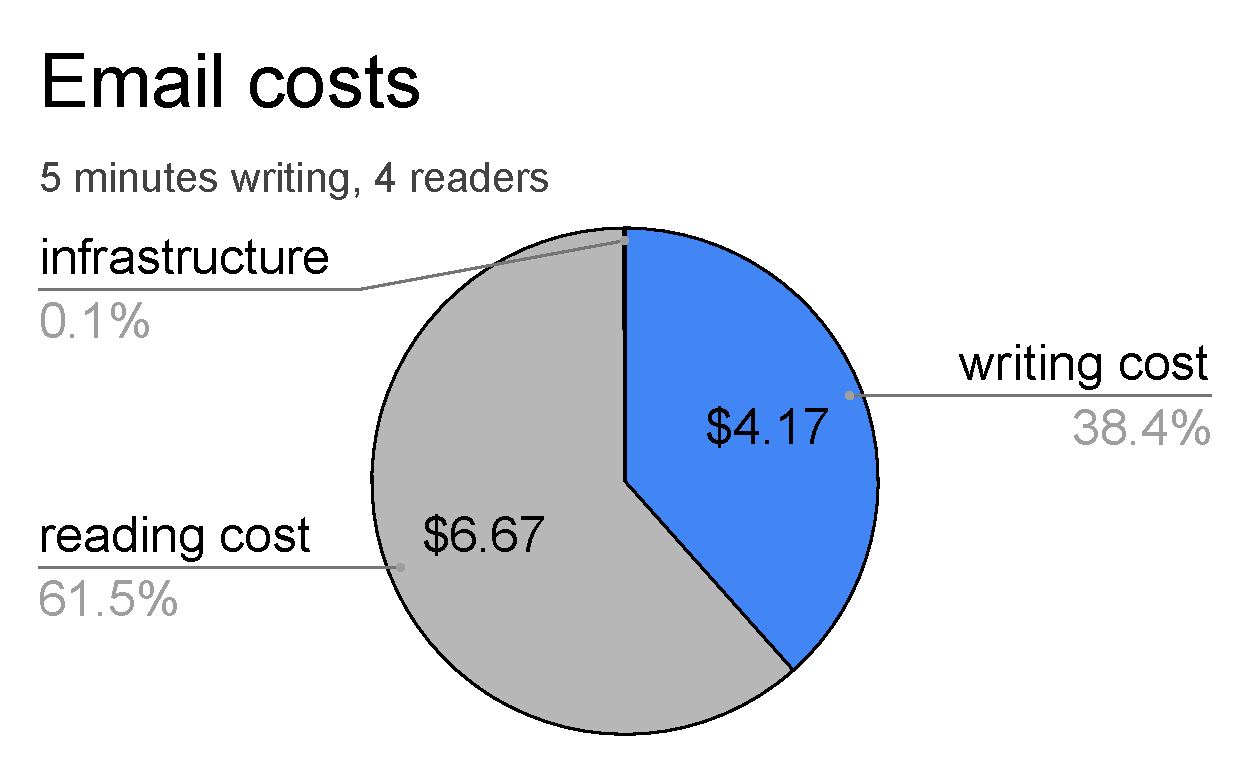
\includegraphics[width=0.7\textwidth]{images/email_costs_5minutes_4people.pdf}
    \caption{Breakdown of costs for Equation~\ref{eq:four_readers}. Assume an hourly rate of \$50 per person, and assume a reading time of 2 minutes.}
    \label{fig:my_label}
\end{figure}

% https://docs.google.com/spreadsheets/d/1ysV5PA3cEcneKv5BViUhAfgNq26cOlNRj6l5fXuHM3Q/edit?usp=sharing


 